\documentclass[a4paper]{article}
\usepackage[newfloat]{minted}
\usepackage{graphicx}
\usepackage{caption}
\usepackage{amsmath}
\usepackage{amsfonts}
\usepackage[a4paper,left=3cm,right=2cm,top=2.5cm,bottom=2.5cm]{geometry}
\usepackage[colorlinks=true, urlcolor=blue, pdfborder={0 0 0}]{hyperref}
\usepackage{subcaption}
\newenvironment{code}{\captionsetup{type=listing}}{}
\SetupFloatingEnvironment{listing}{name=Code}

\title{RL Homework 3}
\author{Ananth Mahadevan}
\begin{document}
\maketitle
\clearpage
\tableofcontents
\clearpage

\section{Question 1}
The heatmap training times for $\epsilon=0.2$ and GLIE is seen in Figure~\ref{fig-training-cartpole}

\begin{figure}[h!]
    \centering
    \begin{subfigure}[b]{0.4\textwidth}
        \centering
        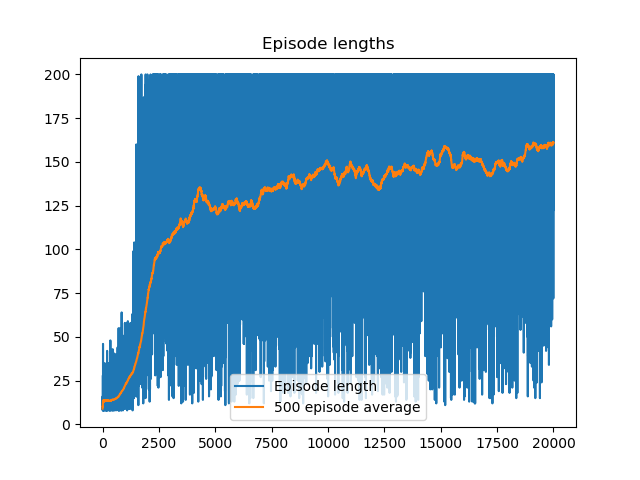
\includegraphics[width=\textwidth]{training_epsilon_0_2.png}
        \caption{$\epsilon=0.2$}
    \end{subfigure}
    \begin{subfigure}[b]{0.4\textwidth}
        \centering
        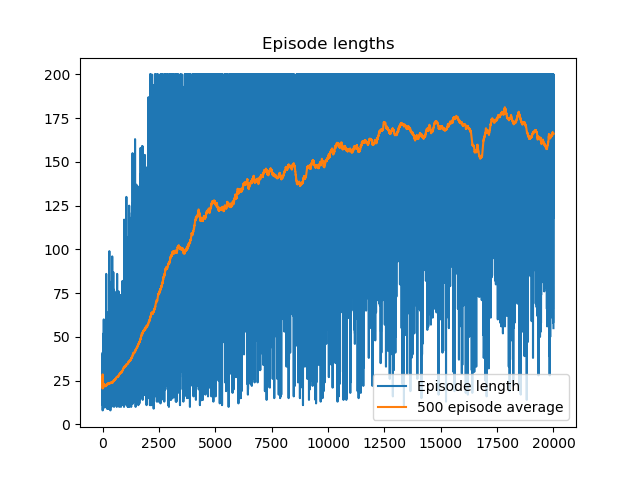
\includegraphics[width=\textwidth]{training_GLIE.png}
        \caption{GLIE}
    \end{subfigure}
    \caption{Training Performance of constant $\epsilon$ and GLIE }
    \label{fig-training-cartpole}
\end{figure}

The heatmap for Task 2 is shown below
\begin{figure}[h!]
    \centering
    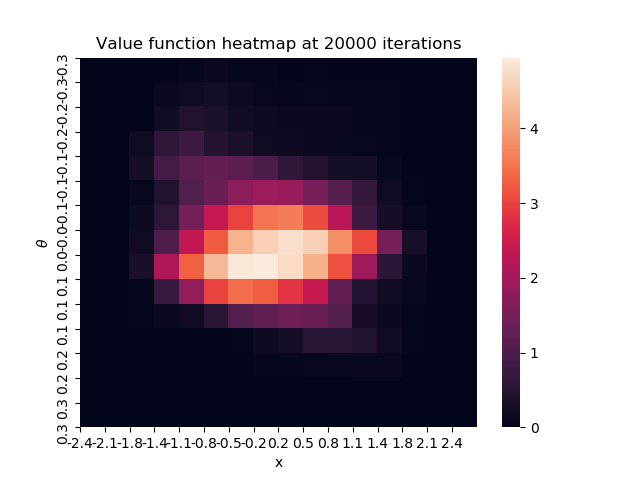
\includegraphics[width=\textwidth]{heatmap_done.png}
    \caption{Heatmap of value function}
    \label{fig-heatmap-done}
\end{figure}

\noindent
My hypothesis for what the heatmap of the value function would have looked like in the various cases are
\begin{itemize}
    \item \textbf{before training} \\ 
    Before training the heatmap would have been randomly close to zero as the value of the Q learning gird would be initialized to zero by a random function.
    \item \textbf{after a single episode}\\
    After a single episode I guess it would update states very close to the center ($x=0$) and small angles. This change in the value will also be very small. This is because the first episode is most likely to fail and hence only the handful of states in which it managed to keep the pole upright would get a reward to have changed the Q learning grid's initial values of 0. And as the rewards would likely be low the change from 0 is also small.
    \item \textbf{Halfway through training}\\
    By this point I would expect the heatmap to more or less converge to roughly how the final heatmap would look. By this I mean that the exploration has been carried out until halfway through, would cover most of the states around the middle of the environment ($x=0$ and $\theta =0$). This is because it has explored most of the state space and as the value of $\epsilon$ is decreasing further the values will not change too much after the halfway point the amount of exploration will decrease and the values will just converge to a better level till the end of the episodes.
\end{itemize}
All of these claims can be verified by the plots of the heatmap as seen in 

\begin{figure}[h!]
    \centering
    \begin{subfigure}[b]{0.4\textwidth}
        \centering
        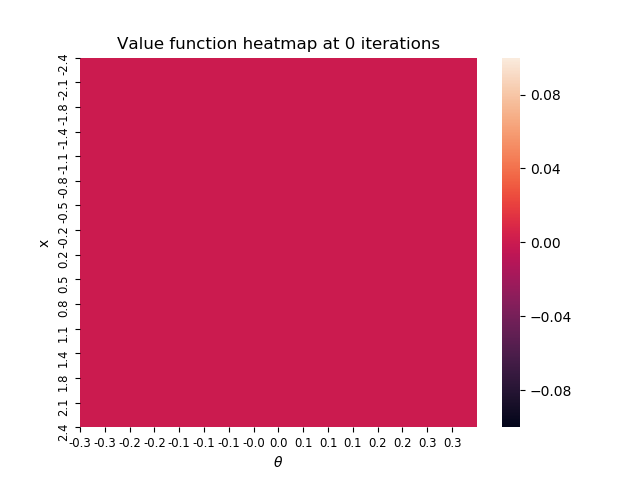
\includegraphics[width=\textwidth]{Heatmap_0.png}
        \caption{After 0 episodes}
    \end{subfigure}
    \centering
    \begin{subfigure}[b]{0.4\textwidth}
        \centering
        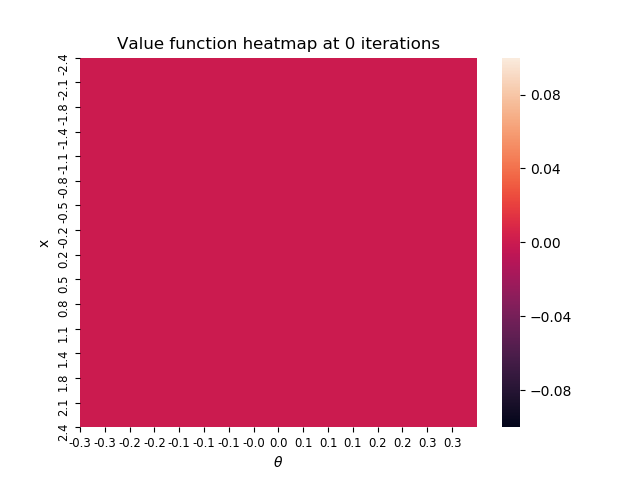
\includegraphics[width=\textwidth]{Heatmap_0.png}
        \caption{After 1 episodes}
    \end{subfigure}

    \begin{subfigure}[b]{0.5\textwidth}
        \centering
        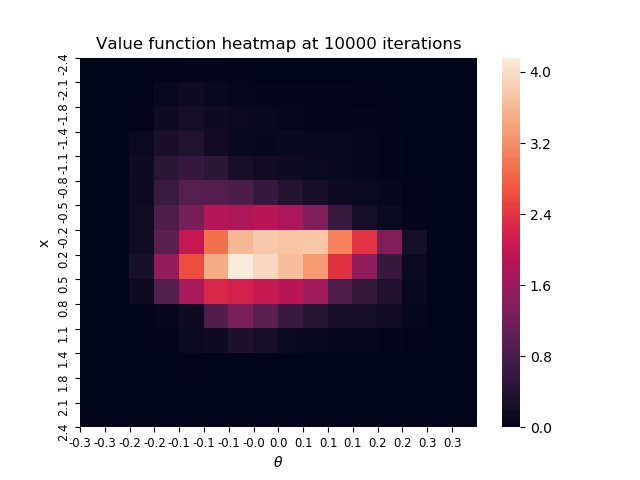
\includegraphics[width=\textwidth]{heatmap_10000.png}
        \caption{After 10,00 episodes (halfway)}
    \end{subfigure}
    \caption{Heatmap of Value function after different number of episodes}
    \label{fig-heatmap-diff}
\end{figure}
\section{Question 2.1}
\section{Question 2.2}
\section{Question 2.3}
\section{Question 3.1}
\section{Question 3.2}

\end{document}